\documentclass{article}
\usepackage[margin=1in]{geometry}
\usepackage{graphicx}
\usepackage{xcolor}
\usepackage{float}
\usepackage{amsmath}
\usepackage{cite}
\usepackage{hyperref}
\usepackage{indentfirst}
\graphicspath{{..} {./images}}

\definecolor{navy-blue}{rgb}{0.22,0.38,0.71}

\renewcommand{\contentsname}{\vspace*{-2\baselineskip}}

\hypersetup{
	colorlinks,
	linkcolor=black,
	urlcolor=blue,
	citecolor=black
}
  		
\begin{document}
\begin{titlepage}
	\centering
	{\huge Lab 8 - SDR: Software Defined Radar}\\[0.25 in]
	
\includegraphics[width=0.6\textwidth]{ua_logo.png}\\[0.25 in]
	{\large \textbf{ECE 531 - Software Defined Radio\\[0.25 in]
	April 28, 2025\\[0.25 in]}}
	{\large Owen Sowatzke, osowatzke@arizona.edu\\[0.05 in]
	Department of Electrical \& Computer Engineering\\[0.05 in]
	University of Arizona, Tucson, AZ 85721\\[0.5 in]}
	\hypersetup{linkcolor=navy-blue}
	\noindent\hrulefill
	\tableofcontents
	\noindent\hrulefill
\end{titlepage}

% \setlength{\parindent}{0pt}

\section{Introduction}
%Introduction to the laboratory experiment, including a brief description of the objectives and goals.

In this lab, we create a monostatic continuous wave (CW) radar using the PlutoSDR. Our CW radar uses the doppler beat frequency to measure velocity and does not measure measure range. We specifically use our CW radar to measure the angular velocity of box fan blades. Then, we explain how we can improve our radar. In the work that follows we provide the procedure for each of our experiments followed by the results. 

\section{Procedure}
% Detailed explanation of the laboratory experiment, including the design, implementation, and testing of the system.

In this section, we provide the procedures for each of our experiments. We specifically use GNU radio to implement a CW radar. A sample CW radar implementation is shown in Figure \ref{fig::gnu_radio_block_diagram}.

\begin{figure}[H]
    	\centering
    \fbox{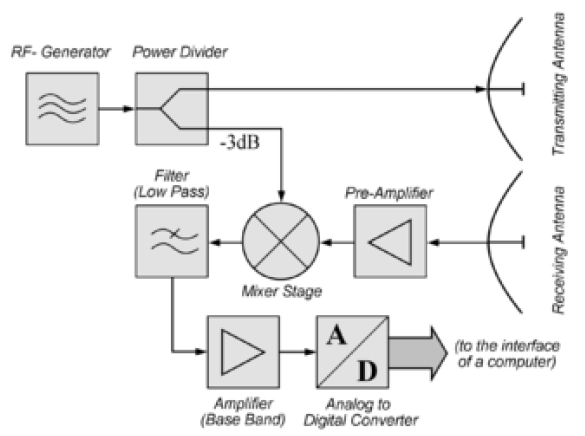
\includegraphics[width=0.5\linewidth]{cw_radar_block_diagram.png}}
    	\caption{RF Block Diagram for a Simple CW Radar \cite{charvat_2011_build}}
    	\label{fig::cw_radar_block_diagram}
\end{figure}

\noindent CW radars, such as the one shown, use the difference between the transmitted and received frequencies to measure the doppler shift of the target.

\begin{equation*}
	f_d = f_r - f_t
\end{equation*}

\noindent For a target with a velocity $v$, the doppler shift can also be approximated as follows:

\begin{equation*}
	f_d \approx \pm\frac{2v}{\lambda}
\end{equation*}

\noindent Here the positive sign corresponds to a closing (approaching) target and the negative sign corresponds to an opening (receding) target. Using the above equation and our measured doppler shifts, we can estimate the target velocity as follows:

\begin{equation*}
	v \approx \pm\frac{f_d\lambda}{2}
\end{equation*}

\noindent Using our CW radar, we specifically measure the angular velocity of a box fan. Next, we explain the strong DC return in our waterfall plots and discuss physical changes that can be made to reduce the power of this return. Then, we discuss how an interfering signal could affect the operation of our radar and propose changes to make the design more resilient to interference. Finally, we discuss how the design can be updated to support range measurements.

\section{Results}
% Results and discussion of the laboratory experiment, including captured outputs, observations, and responses to laboratory questions.

In this section, we provide the results for each of our experiments. We specifically create GNU radio flowchart which implements a CW radio in our PlutoSDR. Next, we use our design to measure the angular velocity of a box fan. Then, we discuss the short-coming of our design: DC return, resilience to interference, and no range measurement. Finally, we discuss how we can improve our design to handle these short-comings.

Our GNU radio flowchart is shown in Figure \ref{fig::gnu_radio_block_diagram}. 

\begin{figure}[H]
    	\centering
    \fbox{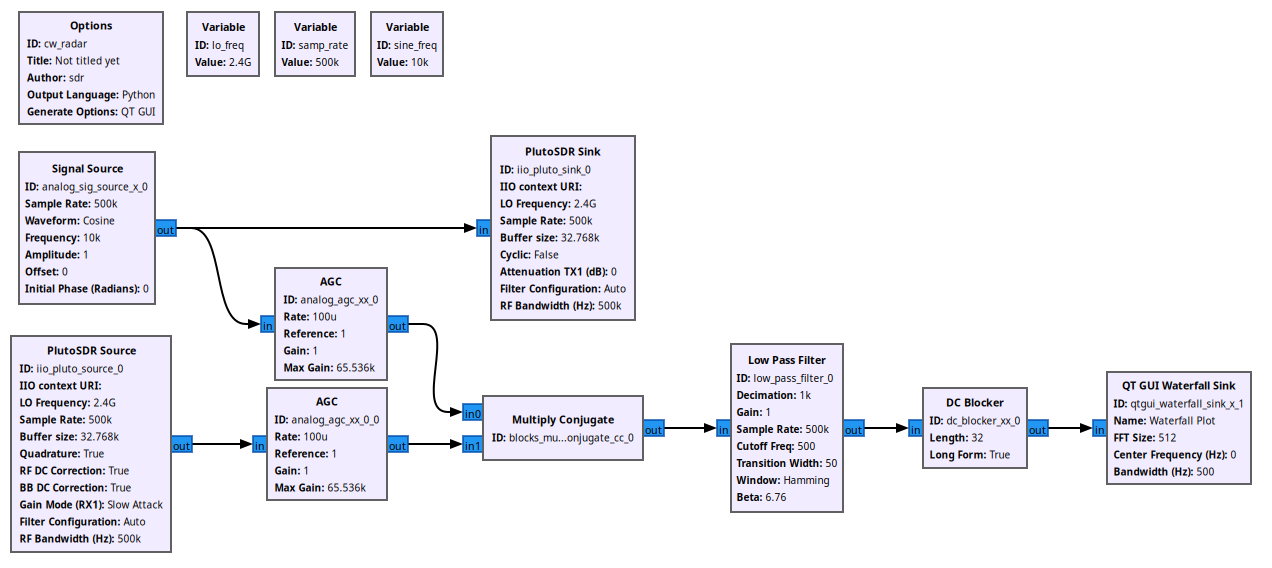
\includegraphics[width=0.7\linewidth]{gnu_radio_block_diagram.png}}
    	\caption{GNU Radio Flowchart which Implements a CW Radar}
    	\label{fig::gnu_radio_block_diagram}
\end{figure}

\noindent In this flowchart, we transmit a 10 kHz sinusoid on a 2.4 GHz carrier frequency. Then, we receive the sinusoid with a 500 kHz sampling rate and RF bandwidth. Note that our sampling greater is much greater than twice the highest frequency in our received signal (10 kHz plus a doppler shift), so we could further reduce our sampling rate if desired. However, if we do so, we should also reduce the RF bandwidth to reduce the amount of noise that aliases back into our spectrum. Next, we perform AGC on the received signal and signal source to maintain signal power. However, both these blocks are optional and can be removed because our transmitted signal has a fixed signal power and because we are performing AGC in the PlutoSDR. Next, we multiply the received signal by the conjugate of the transmitted signal. This is equivalent to mixing our return down to DC. After we mix down, we should be left with a tone at DC (from clutter and leakage) and a tone at the doppler shift. The doppler shift of our returns will be small with respect to our bandwidth. As such we select a sampling rate of 500 Hz for our waterfall plot, which allows us to unambiguously resolve doppler shifts up to $\pm 250\ \text{Hz}$ and radial velocities up to $\pm 15.625 \text{m}/\text{s}$. We use a low-pass filter with decimation to get down to this reduced sample rate. We also use a DC blocker to remove the clutter and leakage returns, which are much stronger than our target return.

%\begin{equation*}
%	f_d = \frac{2v}{\lambda}
%\end{equation*}

% \noindent We specifically choose  shift of 

If we point our PlutoSDR at a running box fan, we receive the waterfall plot generated in Figure \ref{fig::dopp_spectrum}. Note that our flowchart shows the doppler shift for three different fan speeds. 

\begin{figure}[H]
    	\centering
    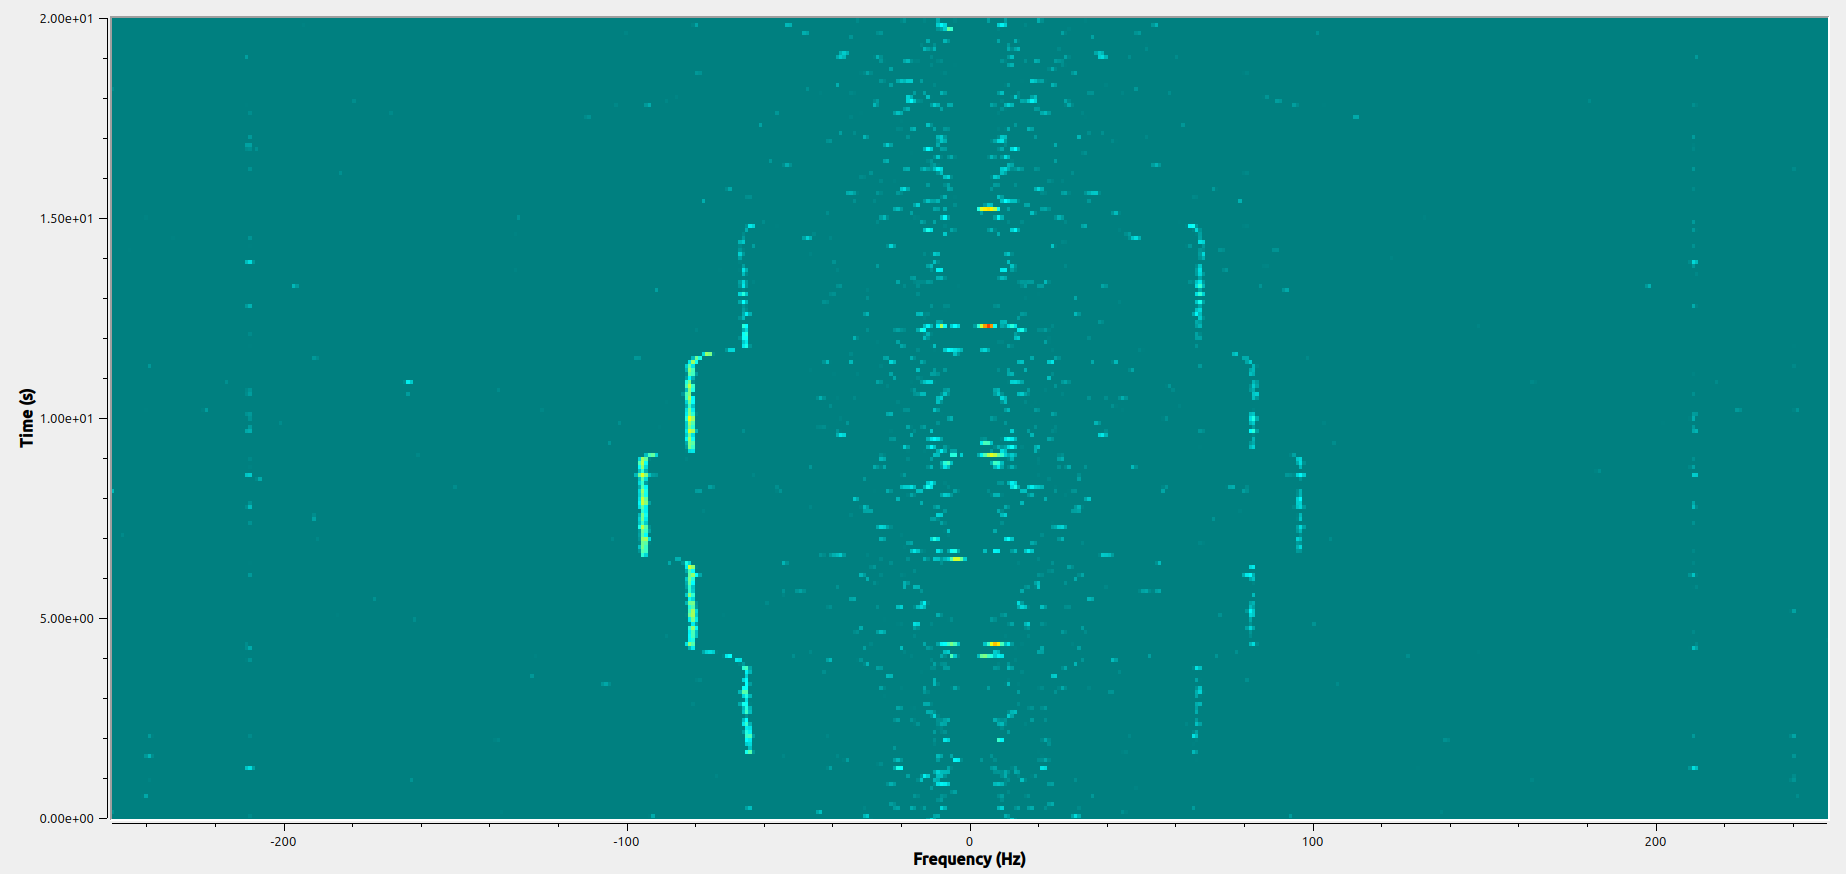
\includegraphics[width=0.9\linewidth]{dopp_spectrum.png}
    	\caption{Waterfall Plot Displaying Doppler Shift from Box Fan}
    	\label{fig::dopp_spectrum}
\end{figure}

\noindent At these fan speeds, we measure doppler shifts of 63 Hz at low fan speeds, 79 Hz at medimum fan speeds, and 95 Hz at high fan speeds. This corresponds to radial velocities of 3.9375 m/s, 4.9375 m/s, and 5.9375 m/s respectively. 12in from fan.

Note that this radar can only sense 

Two common causes of the DC return in our data are clutter (from stationary returns) and transmitter leakage. We can minimize clutter with a tighter antenna pattern or by operating in an controlled environment, such as an anechoic chamber. However, it is usually not possible for us to constrain our environment. Antenna isolation achieved through a tighter antenna pattern or other techniques can be help us achieve better antenna isolation. We can also consider other design such as pulsed doppler radars. However, these radars may not be applicable in all cases (especially with close targets). In the lab, we used a notch filter to remove DC. However, we could have also removed or ignored the offending doppler bins in post-processing.

An interfering signal would negatively impact the CW radar operation. If it was a wideband signal (such as 802.11 WiFi), it could mask the entire bandwidth of our signal and make detection more difficult. Conversely, if the interfering signal was narrow (worse case a tone), it could lead to false detections. To mitigate interference, we should try to minimize the utilized bandwidth. In the sample flowchart, provided in the lab, the RF bandwidth was larger than the sample rate. Tightening the RF bandwidth could prevent interference from aliasing into our bandwidth. Additionally, if the interference is high power, tightening our RF bandwidth can prevent the AGC from acting on interference and increase the effective number of bits for our return. We can also implement more sophisticated techniques to mitigate interference. For example, we can use a coded waveform such as a Barker code or Zadoff-chu waveform to increase the coherent gain on our returns. Additionally, having a tighter antenna pattern can reduce the interference power and increase the power of returns. If we had a ULA, we could even implement beamforming to null signals from specific directions of arrival.

We can extend our design to compute range measurements if we replace our sinusoid with a chirp. This is done in FMCW radars, for example, which we illustrate in Figure \ref{fig::fmcw_radar}

\begin{figure}[H]
    	\centering
    	\fbox{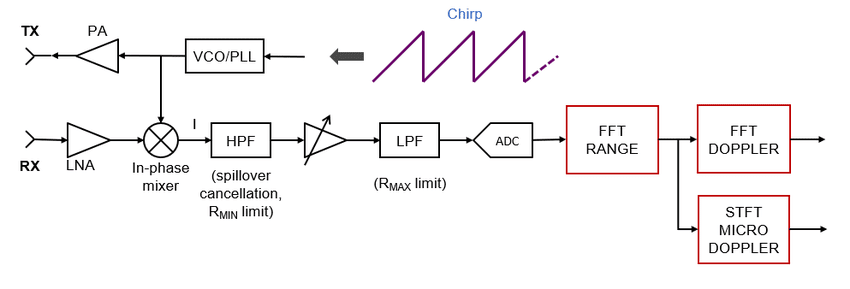
\includegraphics[width=0.6\linewidth]{FMCW Blockdiagram}}
    	\caption{Typical FMCW Block Diagram \cite{9613183}}
    	\label{fig::fmcw_radar}
\end{figure}
	
\noindent In an FMCW radar, we generate our chirp waveform with a VCO.  Typical transmit and receive signals are shown in Figure \ref{fig::fmcw_spectrogram}.

\begin{figure}[H]
    	\centering
    	\fbox{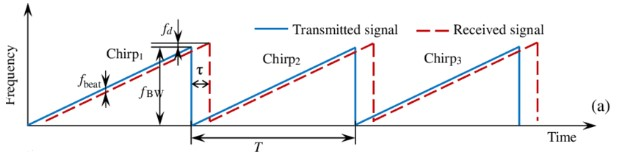
\includegraphics[width=0.6\linewidth]{FMCW Freq-Time graph}}
    	\caption{Time Frequency Plot for Transmit and Receive Signal.\cite{Long2019AssistingTV}}
    	\label{fig::fmcw_spectrogram}
\end{figure}

\noindent After mixing we get a tone with a frequency that is proportional to range. If we limit the maximum resolvable range, we can use a sample rate that is much smaller than the chirp bandwidth, which allows us to use much cheaper hardware. As shown in Figure \ref{fig::fmcw_radar}, we can then use an FFT to detect range. Additionally, we can resolve doppler by taking a slow-time FFT across pulses.

\section{Conclusion}
% Conclusions to the overall lab that discuss meaningful lessons learned and other takeaways from the assignment. (Important)

\bibliographystyle{IEEEtran}
\bibliography{sources}{}

\end{document}